% --------------------------------------------------------------------------
% Version 3.0
% This template is available on the sites:
% https://www.overleaf.com/read/rpkkfchcnbsc
% https://www.overleaf.com/latex/templates/itmo-beamer-theme/fpttrgnmqwsb
% https://github.com/AlexZabashta/ITMO-Beamer-theme
% --------------------------------------------------------------------------

% Attention!!!
% This document was created only as an example of using ITMO beamer styling.
% Don't use it as a Latex or beamer tutorial!
% Check out the capabilities of Latex and beamer (at least basic) independently.


\documentclass[aspectratio=169]{beamer}
\usepackage{ITMOtheme}
\usepackage{tikz}


% Use this package to automatically format references.
% \usepackage[style=mla]{biblatex}
% \addbibresource{references.bib}


%\titlegraphic{\includegraphics[width=0.2\textwidth]}

% The fields 'title', 'author', 'subject', 'keywords' are used to generate a PDF document.
% It is recommended that you fill them in, even if you are creating your title slide manually.

% use \title[short title]{full title}
\title[ITMO LaTex]{\textbf{Networking Fundamentals Presentation}}

%\subtitle[short subtitle]{long subtitle}

\author[LastName F.]{Hemadri Shekhar Das}

\institute[short institute]{Chennai Mathematical Institute}

\where{Chennai}
\date{\today}


\subject{example}
\keywords{ITMO University, LaTex teamplate, beamer}



\begin{document}


% [plain] - modifier to create a blank slide (without bottom bar).
% Ideal for creating the first (title) and last slide with a polygonal background,
% or for transitional slides between chapters or slides with a table of contents.

% \titlepage - command for automatic generation of title slide content.

\begin{frame}[plain]
    \titlepage
\end{frame}

% You can use custom title, if you want.
% Or you can you modify the .sty file.


\begin{frame}[plain]
	\itmobackgroundsnakes{
	\vfill
		%
\includegraphics[width=0.2\textwidth]{itmo/logo_basic_english_white.pdf}
	\vfill
		\usebeamerfont{title}{  \inserttitle\par} 
	\vfill
		Assignment 3 Presentation
	\vfill
		\insertauthor\par
	\vfill
		\insertplace  \;  \insertdate
}
\end{frame}


% Avoid making a table of contents in short presentations.
% Transitions between chapters are best done manually.

%\AtBeginSection[]
%{
%    \begin{frame}[plain]
%        \frametitle{Outline}
%        \Large
%        \tableofcontents[currentsection]
%    \end{frame}
%}


\begin{frame}{Topics Covered}

\begin{itemize}
    \item ICMP - What, Why, How?
    \item Ping 
    \item Traceroute 
\end{itemize}

\end{frame}



\section{First Section}

\subsection{Subsection Example} 

\begin{frame}
\frametitle{ICMP - What, Why, How?}
\begin{itemize}
    \item The Internet Control Message Protocol\textbf{(ICMP)} was conceived as a vital component of the \textbf{Internet Protocol Suite}, introduced in 1981 with RFC 792.
    \item \textbf{The main purpose of ICMP is to \textcolor{red}{report errors}}. 
    \item For instance, if a problem is occurring because the packets of data are too large, and the router is not capable of handling them, the router is going to discard the data packets and send an ICMP message to the sender. That way, it informs the sending device of the issue.
    \item \textbf{ICMP is commonly used as a diagnostic tool.}
\end{itemize}

\end{frame}


\section{Second Section} 

\begin{frame}
\frametitle{ICMP - What, Why, How?}
\textbf{Traceroute} and \textbf{Ping}, are two popular utilities that use \textbf{ICMP}. They both send messages regarding whether data was successfully transmitted.
\begin{block}{Ping}
The Ping command tests the \textbf{speed} of the connection between two different points, and in the report, we can see precisely \textbf{how long it takes} a packet of data to reach its target and return to the sender’s device.
\end{block}

\begin{block}{Traceroute}
The Traceroute command shows the \textbf{actual physical path of the connected routers} that handle and pass the request until it reaches its target destination. Each trip from one router to another is called a \textbf{“hop.”} The Traceroute command also reveals how much time it took for each hop along the way. 
\end{block}

%\begin{alertblock}{Alert Block}
%Suspendisse tincidunt sagittis gravida. Curabitur condimentum, enim sed venenatis rutrum, ipsum neque consectetur orci, sed blandit justo nisi ac lacus.
%\end{alertblock}
\end{frame}

\begin{frame}
\frametitle{ICMP - What, Why, How?}

\begin{itemize}
    \item Internet Control Message Protocol\textbf{(ICMP)} stands as one of the leading protocols of the IP suite.
    \item \textbf{BUT,} it is not associated with any transport layer protocol, like \textbf{TCP} or \textbf{UDP}.
    \item ICMP is one of the \textbf{connectionless protocols}, like UDP.
    
\end{itemize}

\centering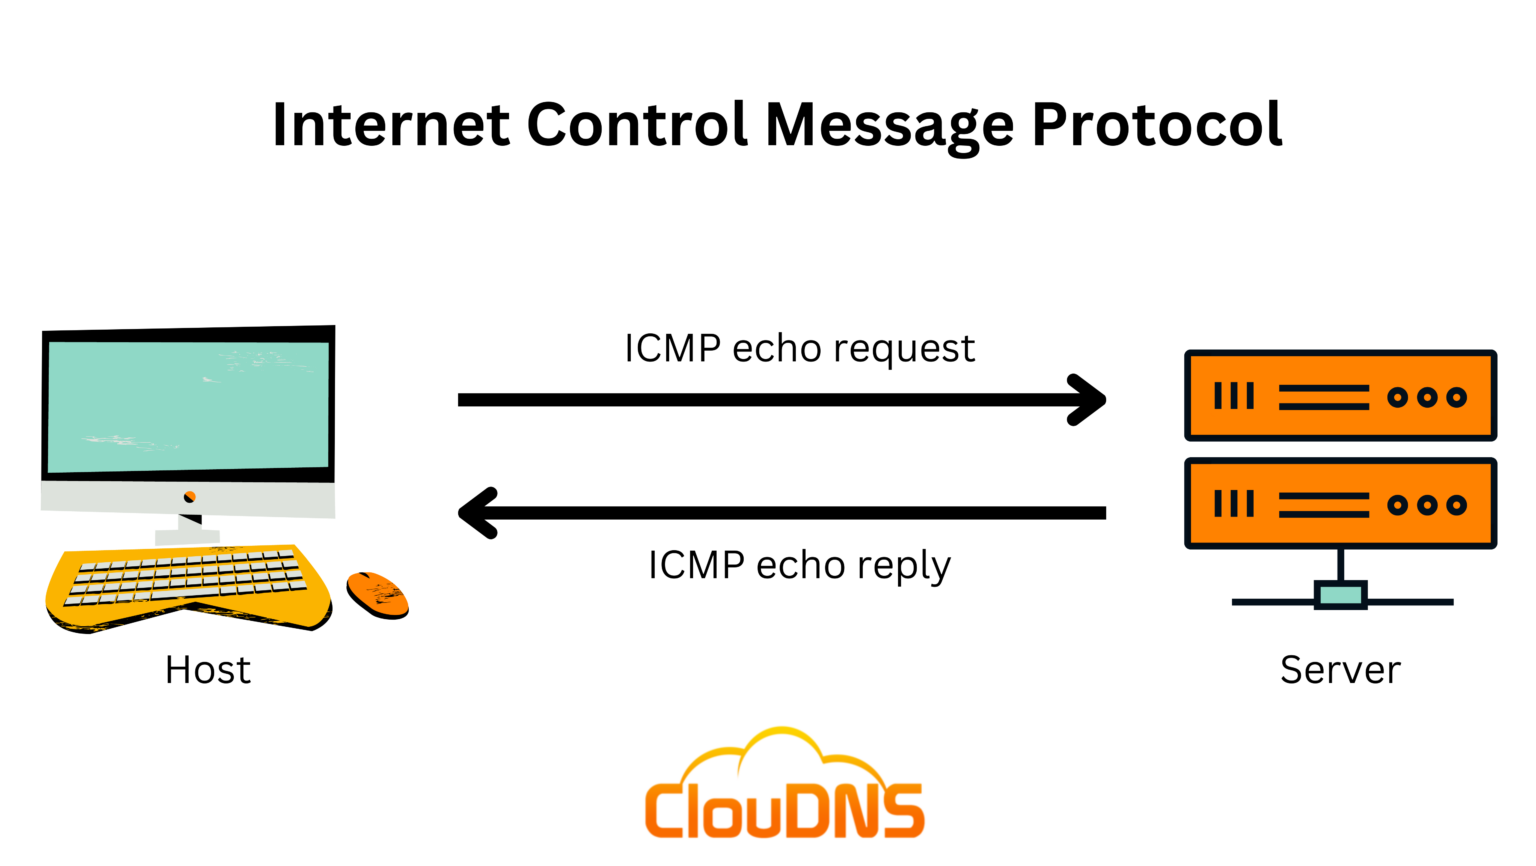
\includegraphics[width=0.9\textwidth]{icmp1.png}

\end{frame}

\begin{frame}
\frametitle{ICMP - What, Why, How?}

\begin{itemize}
    \item All ICMP messages are sent as \textbf{datagrams} and include an \textbf{IP header} that holds the ICMP data.
    \item  ICMP packets are \textbf{IP packets} with ICMP in the \textbf{IP data part.}
    \item ICMP messages also \textbf{include the complete IP header} from the original message. That way, the target system understands which precise packet failed.
    \item ICMP is designed to be used \textbf{within IP} packets.
\end{itemize}

\centering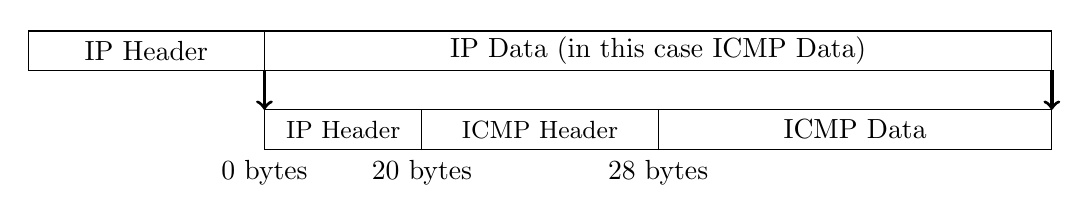
\begin{tikzpicture}

\draw (3,-1.3) node{0 bytes};
\draw (5,-1.3) node{20 bytes};
\draw (8,-1.3) node{28 bytes};


\draw (0,0) rectangle (13,0.5);%IP
\draw (3,0) -- (3,0.5);
\draw (3,-0.5) rectangle (13,-1);%ICMP
\draw (5,-0.5) -- (5,-1);
\draw (1.5,0.25) node{IP Header};
\draw (8,0.25) node{IP Data (in this case  ICMP Data)};
\draw[->,very thick] (3,0) -- (3,-0.5);
\draw[->,very thick] (13,0) -- (13,-0.5);
\draw (8,-0.5) -- (8,-1);
\draw (4,-0.75) node{\small{IP Header}};
\draw (6.5,-0.75) node{\small{ICMP Header}};
\draw (10.5,-0.75) node{ICMP Data};
\end{tikzpicture}

\end{frame}

\begin{frame}
\frametitle{ICMP - What, Why, How?}

\begin{itemize}
    \item In the ICMP packet format, the first 32 bits \textbf{(4 bytes)} of the packet are divided into three fields:
    \begin{itemize}
        \item \textbf{Type}(8-bit)
        \item \textbf{Code}(8-bit) 
        \item \textbf{Checksum}(16-bit)
    \end{itemize}
\end{itemize}

\centering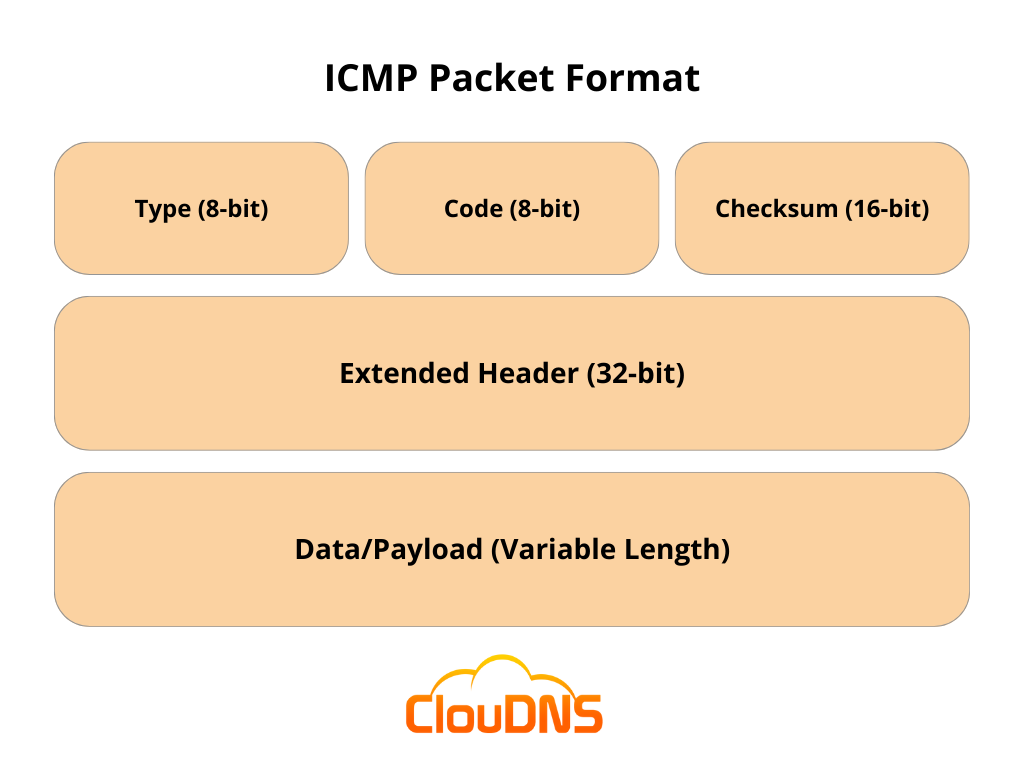
\includegraphics[width=0.64\textwidth]{ICMP-2.png}

\end{frame}

\begin{frame}
\frametitle{Ping}

\begin{itemize}
    \item  \textbf{"Ping"} sends Internet Control Message Protocol (ICMP) packets to the destination.
    \item Then it waits for the echo reply \textbf{"Pong"}.
    \item It can show statistic for this request, errors and packet loss.
\end{itemize}

\begin{alertblock}{Heads-Up}Since most of the code for this assignment was already given, we need to follow the used protocol.\end{alertblock}

We are using the \textbf{Extended Header} for \textbf{ID} and \textbf{Sequence}.

\end{frame}

\begin{frame}
\frametitle{Ping}

\begin{itemize}
    \item \textbf{checksum(data)} : Calculates the checksum of the data
    \item \textbf{receiveOnePing(mySocket, ID, timeout, destAddr)} : To receive the echo reply
    \item \textbf{sendOnePing(mySocket, destAddr, ID)} : To send the echo request
    \item \textbf{doOnePing(destAddr, timeout)} : To call sendOnePing() and receiveOnePing()
    \item \textbf{ping(host, timeout=1)} : To  call doOnePing() with the IP address of the host we want to ping with.
\end{itemize}

\end{frame}

{ % all template changes are local to this group.
    \setbeamertemplate{navigation symbols}{}
    \begin{frame}<article:0>[plain]
        \begin{tikzpicture}[remember picture,overlay]
            \node[at=(current page.center)] {
                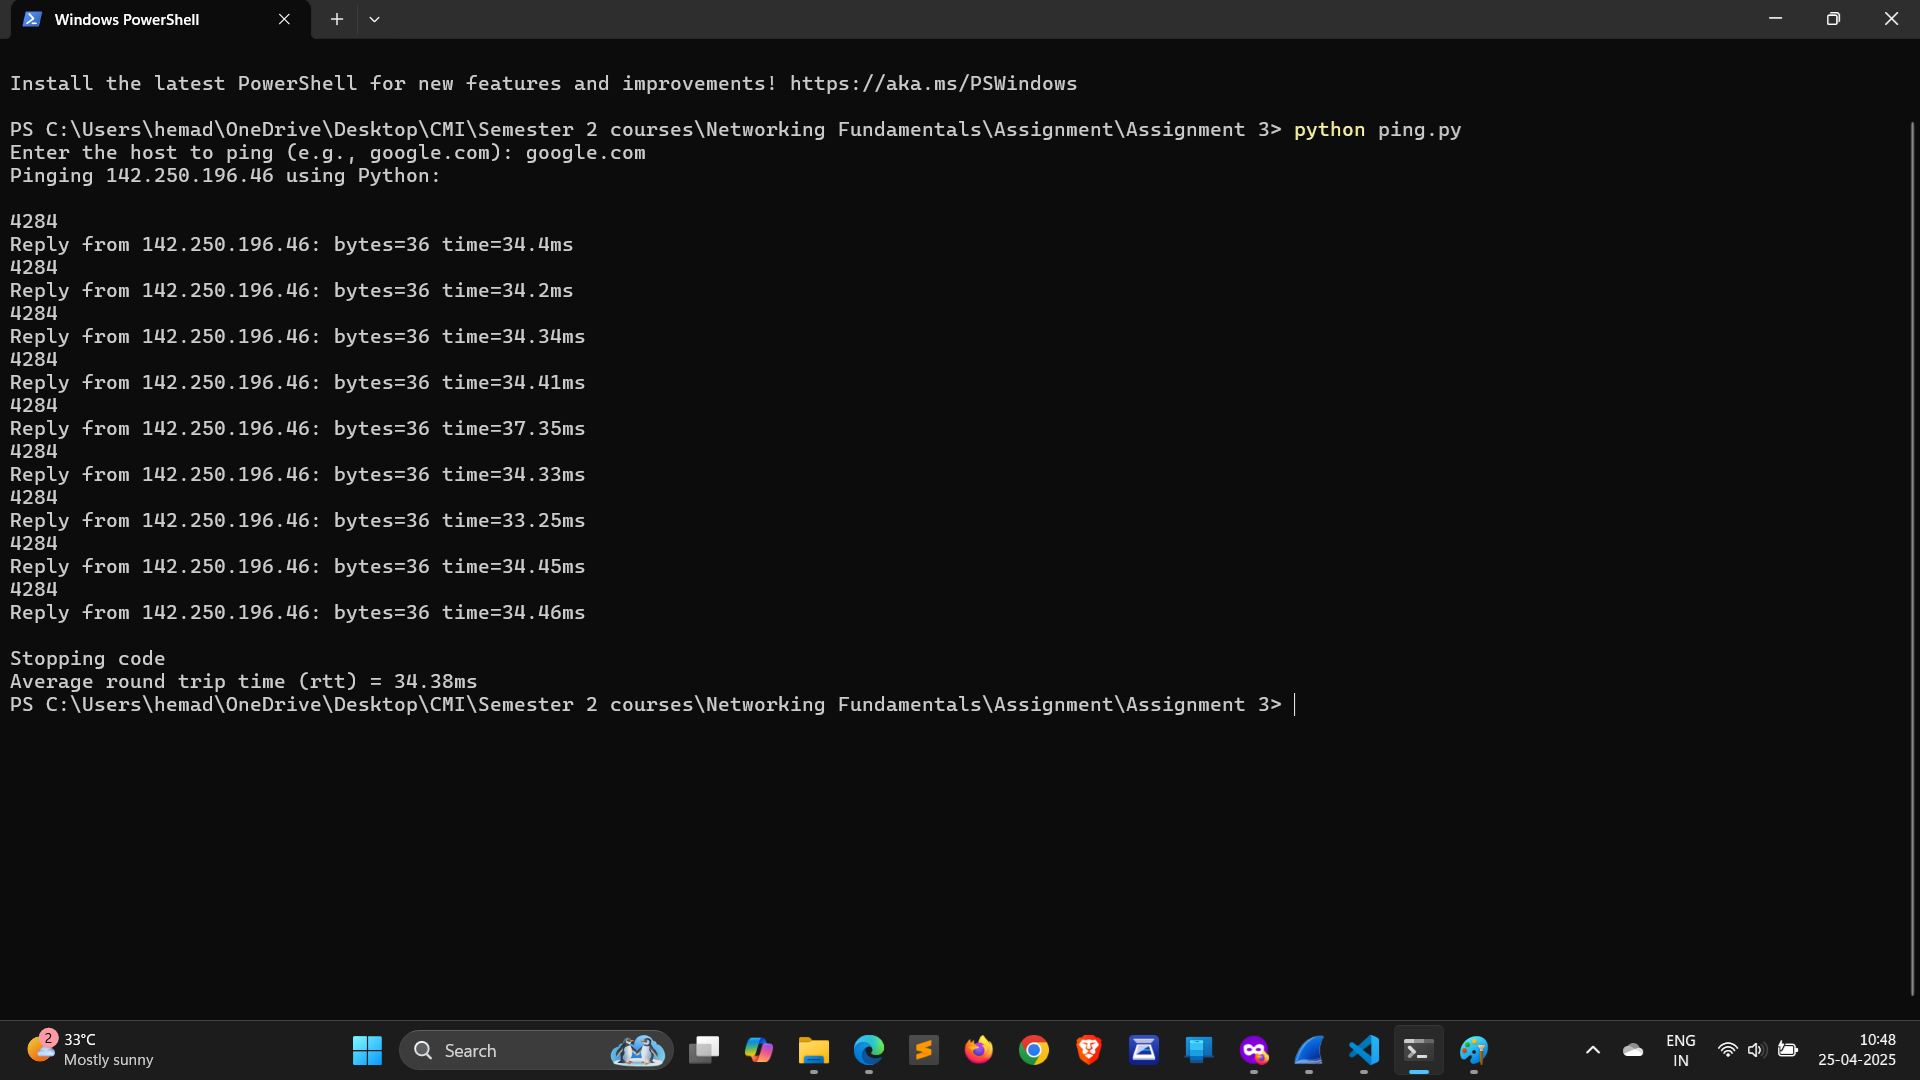
\includegraphics[keepaspectratio,
                                 width=\paperwidth,
                                 height=\paperheight]{ping cmd.png}
            };
        \end{tikzpicture}
     \end{frame}
}

{ % all template changes are local to this group.
    \setbeamertemplate{navigation symbols}{}
    \begin{frame}<article:0>[plain]
        \begin{tikzpicture}[remember picture,overlay]
            \node[at=(current page.center)] {
                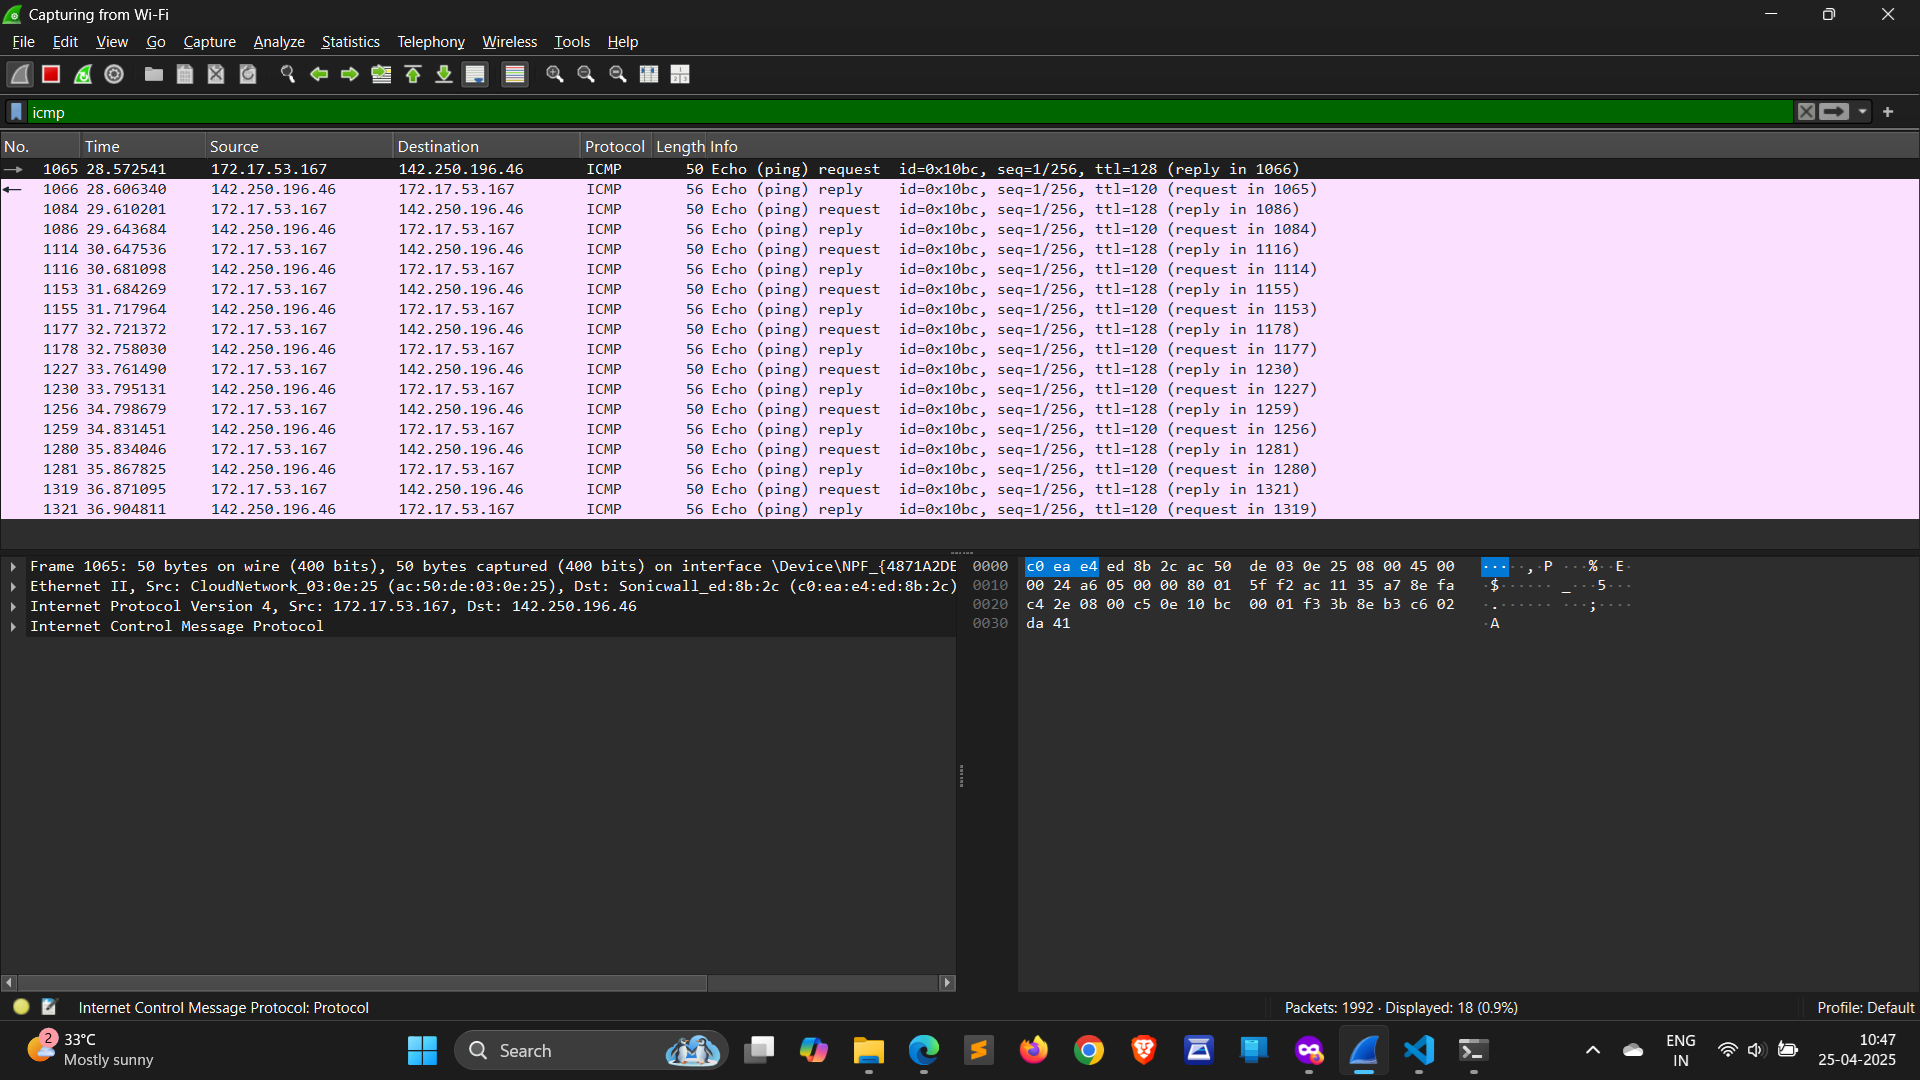
\includegraphics[keepaspectratio,
                                 width=\paperwidth,
                                 height=\paperheight]{ping wireshark.png}
            };
        \end{tikzpicture}
     \end{frame}
}


\begin{frame}
\frametitle{Traceroute}

\begin{itemize}
    \item It is used for checking the route from a computer to a hostname or an IP address.
    \item The \textbf{Traceroute} program sends packets with increasing TTL until we get reply from our target.
\end{itemize}

\centering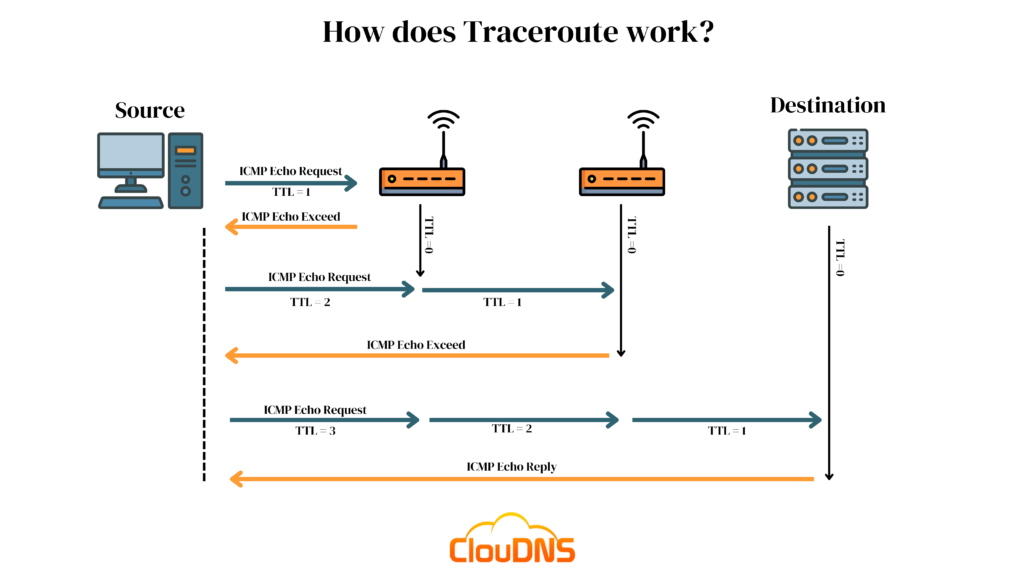
\includegraphics[width=0.93\textwidth]{Trace.png}

\end{frame}

\begin{frame}
\frametitle{Traceroute}

\begin{itemize}
    \item \textbf{checksum(data)} : Calculates the checksum of the data
    \item \textbf{build\_packet()} : To build the icmp packet
    \item \textbf{get\_route(hostname)} : To send the icmp packets with increasing TTL and print the IP addresses of the routers it got the ICMP Time Exceeded Message (TEM) from.
    
\end{itemize}

\end{frame}

{ % all template changes are local to this group.
    \setbeamertemplate{navigation symbols}{}
    \begin{frame}<article:0>[plain]
        \begin{tikzpicture}[remember picture,overlay]
            \node[at=(current page.center)] {
                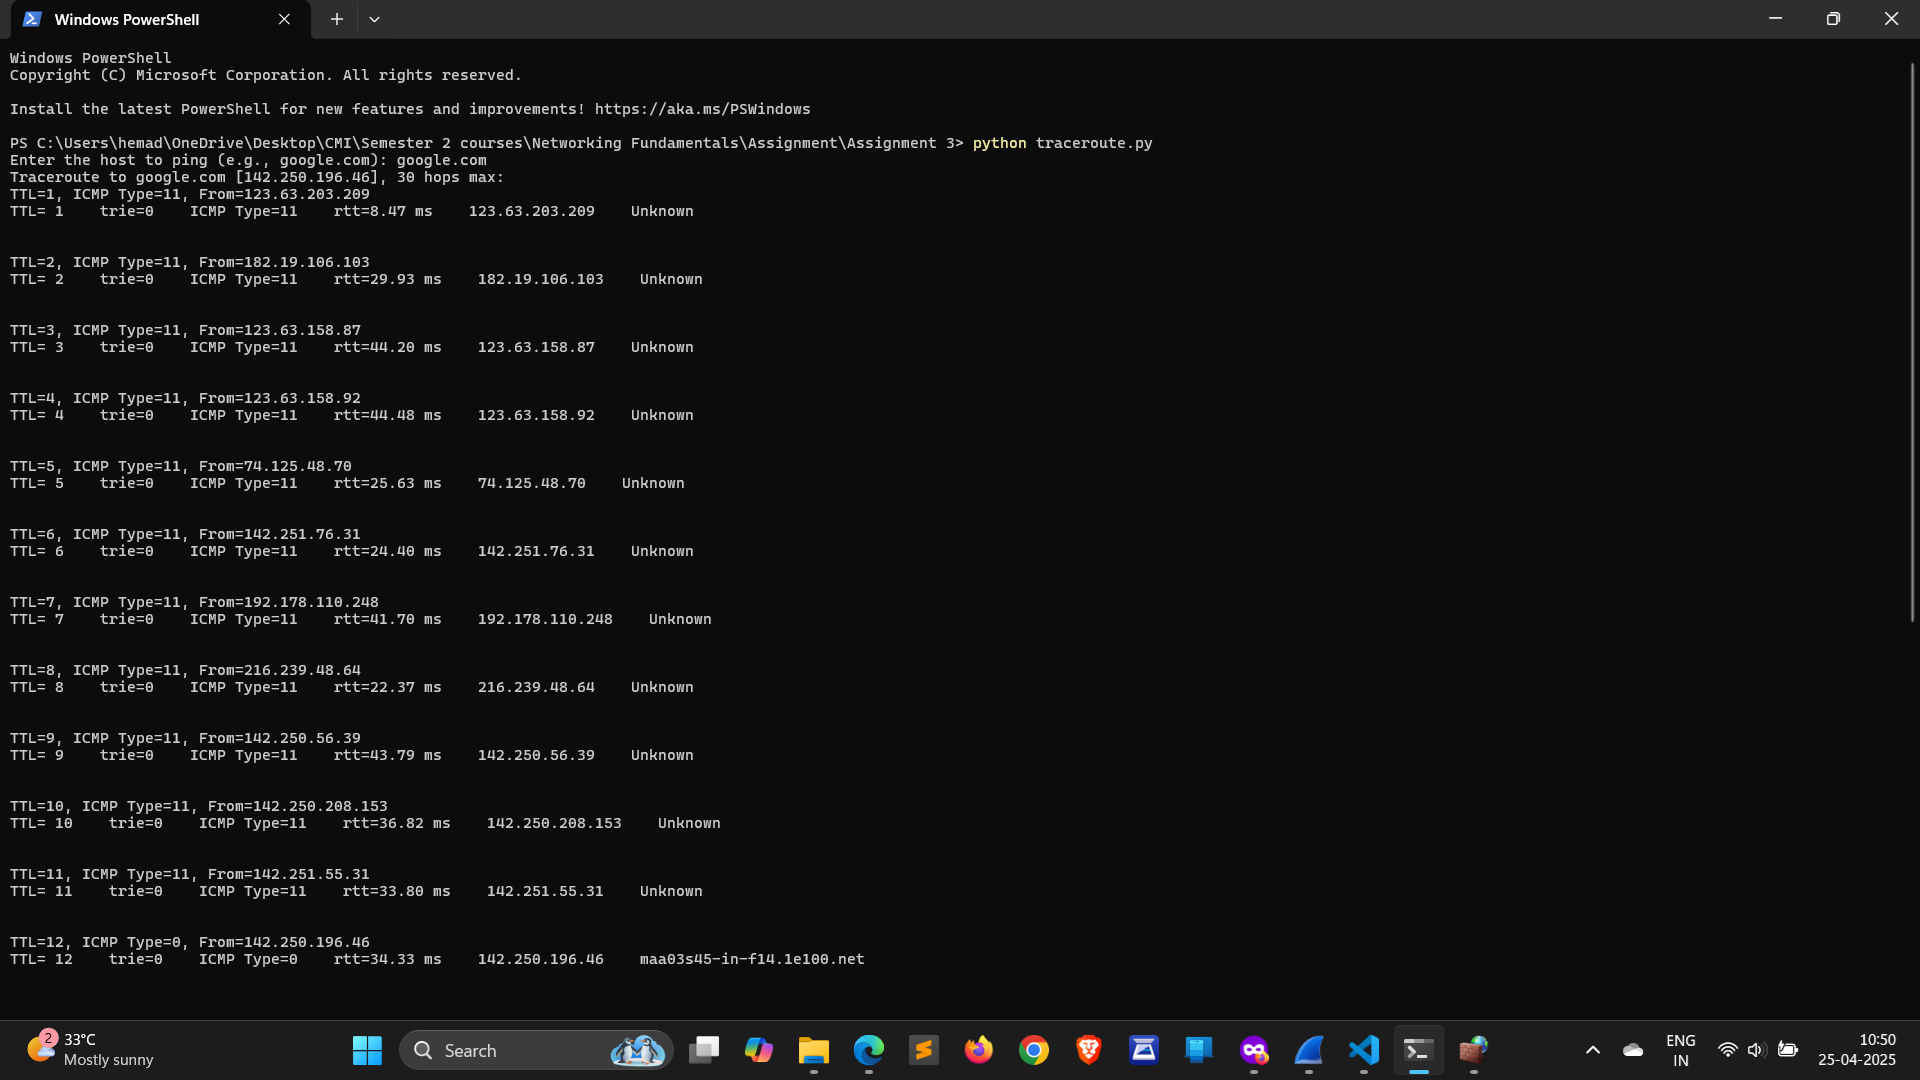
\includegraphics[keepaspectratio,
                                 width=\paperwidth,
                                 height=\paperheight]{traceroute cmd.png}
            };
        \end{tikzpicture}
     \end{frame}
}

{ % all template changes are local to this group.
    \setbeamertemplate{navigation symbols}{}
    \begin{frame}<article:0>[plain]
        \begin{tikzpicture}[remember picture,overlay]
            \node[at=(current page.center)] {
                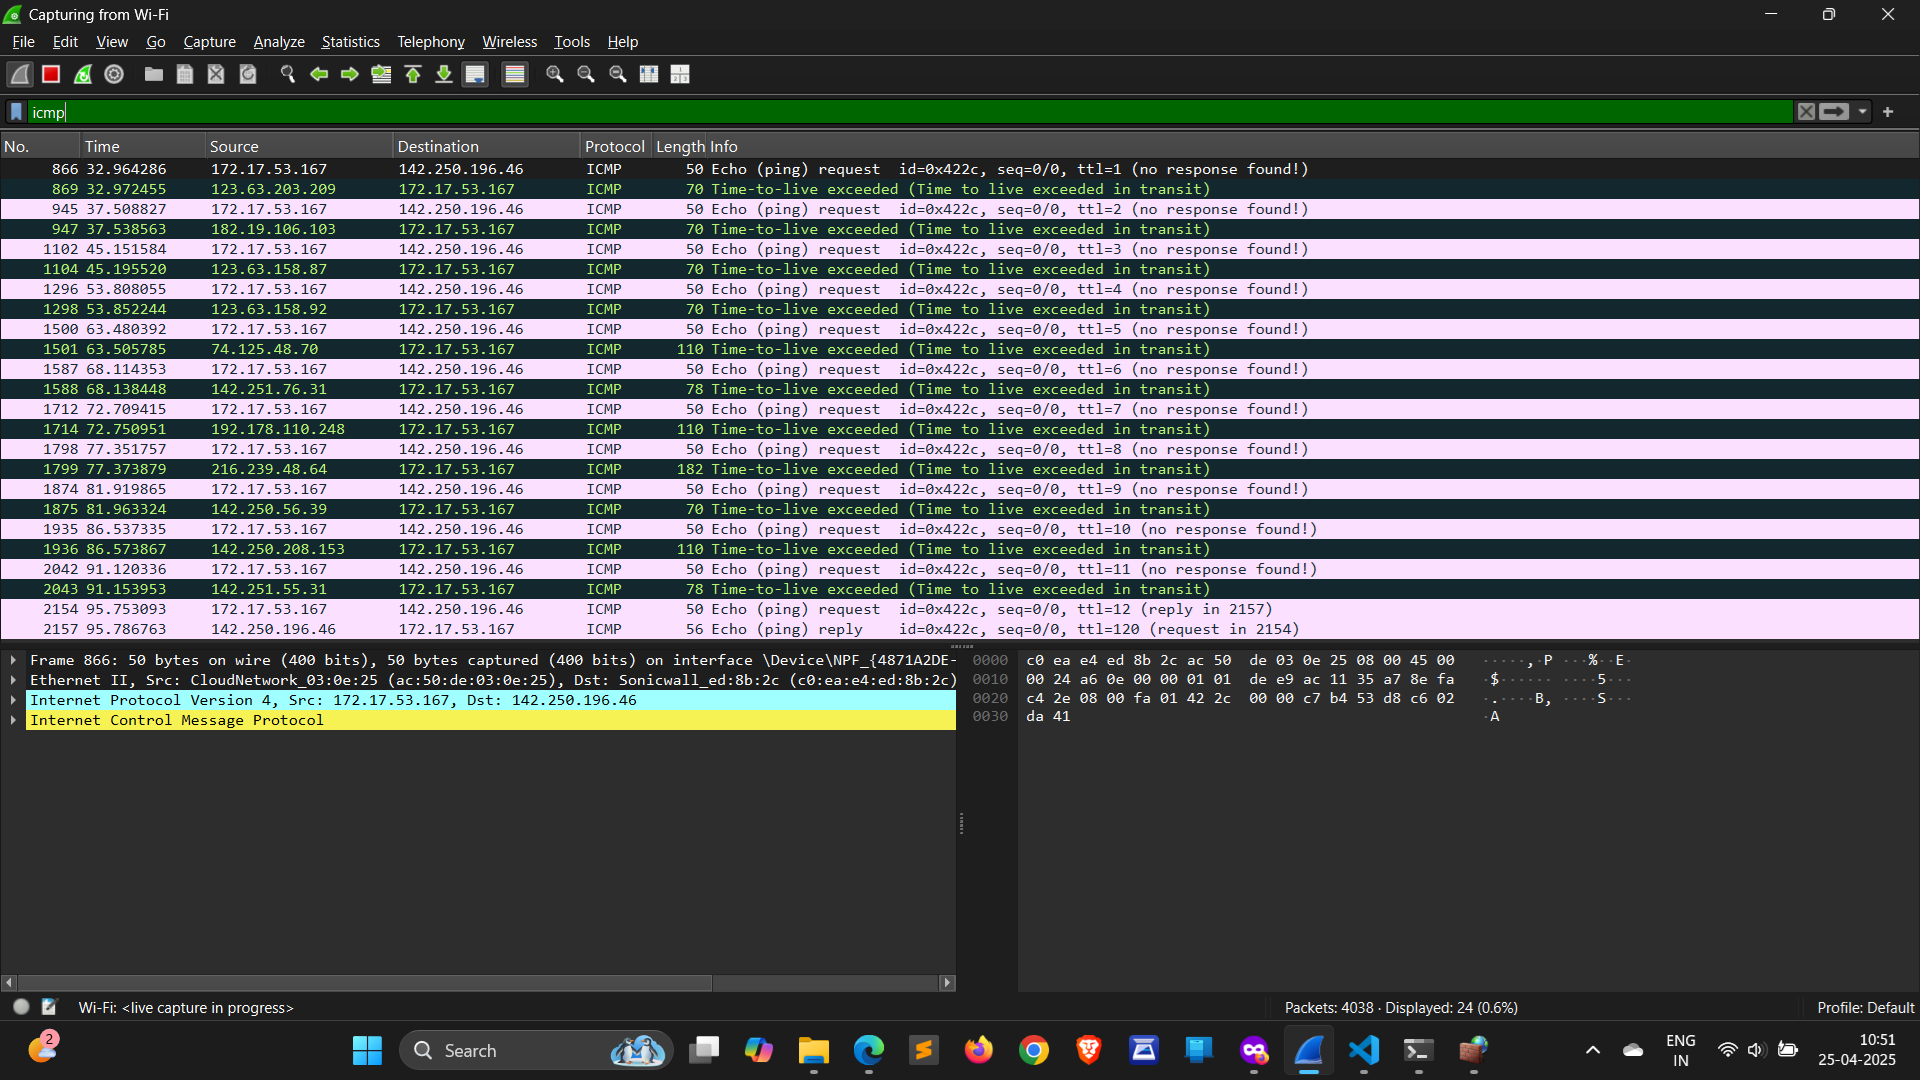
\includegraphics[keepaspectratio,
                                 width=\paperwidth,
                                 height=\paperheight]{traceroute wireshark.png}
            };
        \end{tikzpicture}
     \end{frame}
}

\begin{frame}[plain]
    \itmobackgroundsnakes{
        \vfill
        \Huge{The End}
        \vfill
        
    }
\end{frame}


\end{document}
